% !TeX spellcheck = en_US

\chapter{Introduction}

\begin{itemize}
	\item study computer science
	\item theoretical informatics
	\item automata theory
	\item value of this theory
	\item typical topics, why typical
	\item why automation
\end{itemize}

This work lays out the theory for a program solving this task. As a consequence, parameters, which are sensible as user input, will be incorporated in problem definitions.
In addition, when evaluating possible algorithms, we will take their usability in a practical use case into account.
Furthermore additional theory will be discussed, to enhance usability.

\section{Preliminaries}

We start with defining preliminary theoretical foundations.

\subsection{Deterministic Finite Automatons}

A 5-tuple $A = (Q, \Sigma, \delta, s, F)$ with $Q$ being a finite set of \emph{states}, $\Sigma$ a finite set of \emph{alphabet symbols}, $\delta \colon\ Q \times \Sigma \to Q$ a \emph{transition function}, $s \in Q$ a \emph{start state} and $F \subseteq Q$ \emph{final states} is called \emph{deterministic finite automaton} (DFA)~\cite[p. 46]{hopcroft01}. From now on $\mathcal{A}$ shall denote the set of all DFAs.

We say $\delta(q,\sigma) = p$ is a transition from $q$ to $p$ using symbol $\sigma$. We define the \emph{extended transition function} $\delta^* : Q \times \Sigma^* \to Q$ of a DFA $A = (Q, \Sigma, \delta, s, F)$ as:
\begin{itemize}
	\item $\delta^*(q,\varepsilon) = q$
	\item $\delta^*(q,w\sigma) = \delta(\delta^*(q,w),\sigma)$ for all $q \in Q$, $w \in \Sigma^*$, $\sigma \in \Sigma$
\end{itemize}
Then, the \emph{language} of that DFA is defined as $L(A) = \{\ w\ |\ \delta^*(w) \in F\ \}$~\cite[pp. 49-50. 52]{hopcroft01}.

Given a state $q \in Q$. We call all transitions $\delta(q', \sigma) = q$ \emph{ingoing} transitions of $q$. All transitions $\delta(q, \sigma) = q'$ are called \emph{outgoing} transitions of $q$. If a transition is of the form $\delta(q, \sigma) = q$, then we say that $q$ has a \emph{loop}.

\begin{definition}\label{ch:1:unreachable-states}
	We say a state $q$ is \emph{(un-)reachable} in an DFA $A$, iff there is (no) a word $w \in \Sigma^*$ such that $\delta^*(s, w) = q$.
\end{definition}

A DFA is called \emph{complete} iff for all states, every symbol of the alphabet is used on an outgoing transition: $\forall q\in Q\colon \forall\sigma\in\Sigma\colon \exists p\in Q\colon \delta(q,\sigma) = p$. Note, that every incomplete DFA can be converted to a complete one by adding a so called \emph{dead state}~\cite[p. 67]{hopcroft01}. The resulting automaton has the same language. We will from now on only work with complete DFAs.

\begin{figure}
	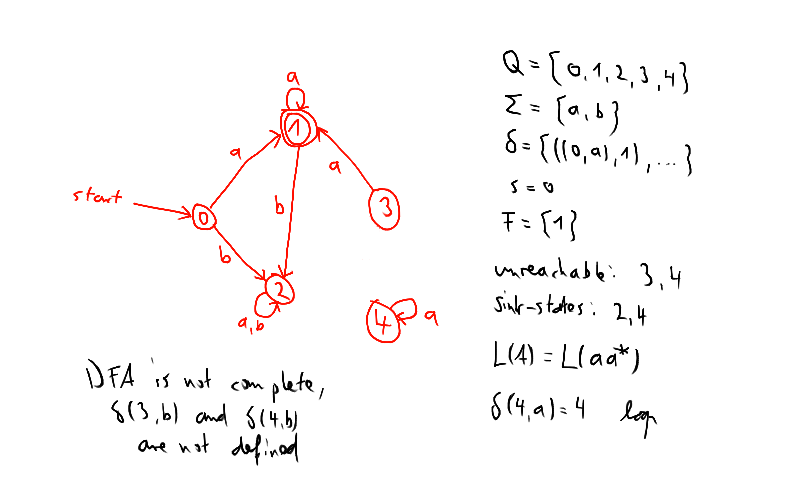
\includegraphics[width=\linewidth]{images/dfa.png}
	\caption{An example DFA and its properties.}
	\label{fig:dfa}
\end{figure}

\subsection{Minimal DFAs}

This section closely follows~\cite[pp. 42-45]{schoening01}. We call a DFA $A$ \emph{minimal}, if there exists no other automaton with the same language using less states. With $\mathcal{A}_{min}$ we shall denote the set of all minimal DFAs.

The \emph{Nerode-relation} $\equiv_L\ \subseteq\ \Sigma^* \times \Sigma^*$ of a language $L$ with alphabet $\Sigma$ is defined as follows:
\begin{displaymath}
	x \equiv_L y\ \Leftrightarrow_{def}\ \forall z\in\Sigma^*\colon (xz\in L \Leftrightarrow yz\in L)
\end{displaymath}
The Nerode-relation of a DFA $A$ is the the Nerode-relation of its language: $\equiv_{L(A)}$. If the context makes it clear, than we will shorten the notation of a equivalence class $[x]_{\equiv_L}$ with $[x]$.

The \emph{equivalence class automaton} $A_L = (Q_L, \Sigma_L, \delta_L, s_L, F_L)$ to a regular language $L$ with alphabet $\Sigma$ is defined as follows:
\begin{itemize}
	\item $Q_L = \{\ [x]\ |\ x \in \Sigma^*\ \}$
	\item $\Sigma_L = \Sigma$
	\item $\delta_L([x], \sigma) = [x\sigma],\ \forall x\in\Sigma^*,\ \forall\sigma\in\Sigma$
	\item $s = [\varepsilon]$
	\item $F = \{\ [x]\ |\ x \in L\ \}$
\end{itemize}
\begin{theorem}
	Given a language $L$, then the equivalence class automaton $A_L$ is minimal.
\end{theorem}

\subsection{Isomorphy of DFAs}

Given two DFAs $A_1 = (Q_1, \Sigma_1, \delta_1, s_1, F_1)$ and $A_2 = (Q_2, \Sigma_2, \delta_2, s_2, F_2)$. We say $A_1$ and $A_2$ are \emph{isomorph} ($A_1 \cong A_2$), iff:
\begin{itemize}
	\item $\Sigma_1 = \Sigma_2$ and
	\item there exists a bijection $\pi\colon Q_1 \to Q_2$ such that:
	
	$\pi(s_1) = s_2$
	
	$\forall q\in Q_1\colon (q\in F_1 \Longleftrightarrow \pi(q)\in F_2)$
	
	$\forall q\in Q_1\colon \forall\sigma\in\Sigma\colon (\pi(\delta_1(q,\sigma))=\delta_2(\pi(q),\sigma))$
\end{itemize}
\begin{theorem} \textnormal{\cite[p. 45]{schoening01}} 
	Every minimal DFA is unique except for isomorphy.
\end{theorem}
\begin{corollary}\label{ch:1:cor:all-min-dfa-ism}
	Every minimal DFA $A$ is isomorph to its corresponding equivalence class automaton $A_{L(A)}$.
	\gregor{All min. DFAs are ism. to each other, including A\_L}
\end{corollary}

\subsection{Duplicate states}

\begin{definition}[Duplicate States]\cite[p. 154]{hopcroft01}
	Two states $q_1, q_2 \in Q$ of a DFA $A = (Q, \Sigma, \delta, s, F)$ are called \emph{duplicates} of each other, iff $d_A(q_1, q_2)$ is true, whereas
	\begin{displaymath}
	q_1\ d_A\ q_2\ \Leftrightarrow_{def}\ \forall z \in \Sigma^* \colon\ (\delta^*(q_1, z) \in F \Leftrightarrow \delta^*(q_2, z) \in F)
	\end{displaymath}
\end{definition}
\noindent Note that the relation $d_A$ is indeed an equivalence relation.

\subsection{The minimization algorithm}

This minimization algorithm requires a complete DFA and works in four major steps, removing essentially states in such a way, that no unreachable and no duplicate states are left.
\begin{enumerate}
	\item Compute all unreachable states via breadth-first search for example.
	
	\vspace{0.2cm}
	\begin{algorithmic}[1]
		\Function{ComputeUnreachableStates}{$A$}
			\State $U \gets Q \setminus \{s\}$	\Comment{undiscovered states}
			\State $O \gets \{s\}$				\Comment{observed states}
			\State $D \gets \{\}$				\Comment{discovered states}
			\While {$|O| > 0$}
				\State $N \gets \{\ p\ | \ \exists q \in O\ \sigma \in \Sigma \colon\ \delta(q, \sigma) = p\ \land\ p \notin O \cup D\ \}$
				\State $U \gets U \setminus N$
				\State $D \gets D \cup O$
				\State $O \gets N$
			\EndWhile
			\State \Return $U$
		\EndFunction
	\end{algorithmic}

	\item Remove all unreachable states and their transitions.
	
	\vspace{0.2cm}
	\begin{algorithmic}[1]
		\Function{RemoveUnreachableStates}{$A, U$}
			\For {$q$ \textbf{in} $U$}
				\If {$q \in F$}
					\State $F \gets F \ \{q\}$
				\EndIf
				\State $\delta \gets \delta \setminus \{\ ((q_1, \sigma), q_2) \in \delta\ |\ q_1 = q \lor q_2 = q\ \}$
			\EndFor
			\State \Return $A$
		\EndFunction
	\end{algorithmic}

	\item Compute all non-duplicate states ($\neg d_A(p, q)$) via the \MinMark-algorithm.
	
	\vspace{0.2cm}
	\begin{algorithmic}[1]
		\Function{\MinMark}{$A$}
		\State $M \gets \{ (p,q), (q,p)\ |\ p \in F, q \notin F \}$
		\Do
			\State $M' \gets \{ (p,q)\ |\ (p,q) \notin M \land \exists \sigma \in \Sigma \colon (\delta(p,\sigma), \delta(q,\sigma)) \in M \}$
			\State $M \gets M \cup M'$
		\doWhile {$M' \neq \emptyset$}
		\State \Return $M$
		\EndFunction
	\end{algorithmic}

	\item Merge all duplicate state pairs, which are exactly those, that are not in $\neg d_A$.
	
	\vspace{0.2cm}
	\begin{algorithmic}[1]
		\Function{\MinMerge}{$A, \neg d_A$}
			\State compute $d_A$
			\While {$d_A \neq \emptyset$}
				\State $(p,q) \in d_A$
				\State $d_A \gets d_A \setminus \{ (p,q) \}$
				\If {$p \neq q$}
					\State exchange all occurrences of $q$ in $A$ and $d_A$ by $p$
				\EndIf
			\EndWhile
			\State \Return $A$
		\EndFunction
	\end{algorithmic}
\end{enumerate}
\begin{theorem}
	The minimization algorithm computes a minimal DFA to its input DFA.
\end{theorem}
\noindent The definition of this DFA minimization algorithm is inspired by Schöning~\cite[p. 46]{schoening01}.

When looking at \MinMark, one notes, that it computes distinct subsets of $Q \times Q$ on the way. Indeed, one could write the algorithm in such a way, that these subsets are explicitly computed in form of a function $m\colon\mathbb{N}\to\mathcal{P}(Q\times Q)$:
\vspace{0.2cm}
\begin{algorithmic}[1]
	\Function{$m$-MinimizationMark}{$(Q, \Sigma, \delta, s, F)$}
	\State $i \gets 0$
	\State $m(0) \gets \{ (p,q), (q,p)\ |\ p \in F, q \notin F \}$
	\Do
		\State $i \gets i + 1$
		\State $m(i) \gets \{ (p,q)\ |\ (p,q) \notin \bigcup{m(\cdot)} \land \exists \sigma \in \Sigma \colon (\delta(p,\sigma), \delta(q,\sigma)) \in m(i-1) \}$
	\doWhile {$m(i) \neq \emptyset$}
	\State \Return $\bigcup{m(\cdot)}$
	\EndFunction
\end{algorithmic}
\vspace{0.2cm}
Using this redefinition, we can easier refer to the state pairs marked in a certain iteration. We will use both variants in exchange.

We will denote the number of iterations done by \MinMark\ on an DFA $A$ as $\mmD(A)$. Note that $\mmD(A) = \max n \in \mathbb{N}\ |\ m(n) \neq \emptyset$.


\section{Requirements analysis}

\subsection{Example of a DFA minimization task for students}

\begin{itemize}
	\item present a typical task and its solution (text, image, table)
	\item name its elements
	\item clarify two parts: solution, task
	\item clarify four parts from task to solution: find unreachables, delete them, find duplicates, merge them
	\item what are the difficulties of this tasks?
\end{itemize}

We will call the minimal automaton \emph{solution DFA} ($A_{sol}$) and its extension with duplicate and unreachable states \emph{task DFA} ($A_{task}$).

heuristic:
\begin{itemize}
	\item $h \colon \mathcal{A} \times \mathcal{A} \to \mathbb{R^+}$
	\item $h(A_{min}, A_{task}) = studentfriendliness$
\end{itemize}

\subsection{Definition and evaluation of possible requirements}

\label{ch:1:determined-requirements}
Dismissed:
\begin{itemize}
	\item $h(A_{sol}, A_{task}) = |Q_{task}|\ /\ |Q_{sol}|$
	\item number of transitions
	\item max degree of a node (Why not this?)
	\item Does GraphViz have a heuristic?
\end{itemize}
Accepted solution DFA criteria:
\begin{itemize}
	\item[->] minimal
	\item[->] number of states
	\item[->] number of \MinMark\ iterations ($\mmD(A_{sol})$)
	\item[->] alphabet size
	\item[->] number of accepting states
	\item[->] planarity (can be checked in $O(|Q_{sol}|)$)
	\item[->] $A_{sol}$ is unused (regarding all previously generated solution DFAs)
	
	\begin{definition}[Unused DFAs] \label{ch:1:unused-dfa}
		A DFA $A$ is \emph{unused} regarding a set of \emph{used DFAs} $U$, if $A$ is not isomorph to any DFA in $U$.
	\end{definition}
\end{itemize}
Accepted task DFA criteria:
\begin{itemize}
	\item[->] $L(A_{sol}) = L(A_{task})$
	\item[->] $\mmD(A_{sol}) = \mmD(A_{task})$
	\item[->] number of duplicate states
	\item[->] number of unreachable states
	\item[->] alphabet size
	\item[->] planarity (can be checked in $O(|Q_{task}|)$)
	\item[->] completeness (for \MinMark-algorithm to work)
\end{itemize}

\section{Approach and general algorithm}

In this work we will first build the solution DFA (step 1), and - based on that - the task DFA by adding duplicate and unreachable states (step 2). Both steps will fulfill all criteria chosen above and are covered in depth in chapter~\ref{ch:2} respectively chapter~\ref{ch:3}.

It follows that $\mmD$ and $L$ of both DFAs will be set when building $A_{sol}$. As a consequence we need to ensure that adding duplicate and unreachable state does neither change $\mmD(A_{task})$ nor $L(A_{task})$ in comparison to $A_{sol}$. We will do this during the discussion of step 2.

Here follow problem definitions for the two steps, which specify all needed informations. \gregor{Hidden formulation here} %The first problem is lain out in a way, such that it does

\begin{definition}[BuildNewMinimalDFA] $ $
	\begin{description}
		
		\item[Given:] $ $
		
		$q, a, f, m_{min}, m_{max} \in \mathbb{N},$
		
		$p \in \{0,1\}$
		\item[Request:] $ $
		
		Let $A_{sol} = (Q, \Sigma, \delta, s, F)$ be a DFA, such that
		
		\qquad $|Q|=q$, $|\Sigma|=a$, $|F|=f$,
		
		\qquad $m_{min} \le \mmD(A_{sol}) \le m_{max}$,
		
		\qquad $A_{sol}$ is planar iff $p = 1$ and
		
		\qquad the language of $L(A)$ is unequal to any DFA used before.
		
		Return $A_{sol}$, if it exists, $\bot$ otherwise.
	\end{description}
\end{definition}

\begin{definition}[ExtendMinimalDFA] $ $
	\begin{description}
		
		\item[Given:] $ $
		
		$A_{sol} = (Q, \Sigma, \delta, s, F) \in \mathcal{A}_{min},$
		
		$p \in \{0,1\},$
		
		$d, u \in \mathbb{N}$
		\item[Request:] $ $
		
		A DFA $A_{task} = (Q', \Sigma', \delta', s', F')$ with reachable duplicate states $q_1 \ldots q_d$ and unreachable states $p_1 \ldots p_u$, such that
		
		$Q = Q' \cup \{ q_1, \ldots q_d, p_1 \ldots p_u \}$,
		
		$\Sigma = \Sigma'$, $s = s'$,
		
		$F \subseteq F'$,
		
		$A_{task}$ is planar iff $p = 1$,
		
		$L(A_{sol}) = L(A_{task})$ and $\mmD(A_{sol}) = \mmD(A_{task})$.
	\end{description}
\end{definition}

\noindent The main algorithm will then simply be:
\vspace{0.2cm}
\begin{algorithmic}[1]
	\Function{GenerateDFAMinimizationProblem}{$q, a, f, m_{min}, m_{max}, p_1, p_2, d, u$}
	\State $A_{sol} \gets \textsc{BuildNewMinimalDFA}(q, a, f, m_{min}, m_{max}, p_1)$
	\State $A_{task} \gets \textsc{ExtendMinimalDFA}(A_{sol}, p_2, d, u)$
	\State \Return $A_{sol}, A_{task}$
	\EndFunction
\end{algorithmic}


